\documentclass[../main.tex]{subfiles}
 
\begin{document}

\section{Wednesday}

Today is the rough day. Your schedule is more or less blocked from noon until 10:30 in the evening. Where your previous days saw either one or two shifts totalling less than six hours of time spent repeating, greeting, or seating attendees, today's schedule has been changed since you last checked it on Monday morning. Surprise! At noon you begin back-to-back shifts in VR Village, followed by a short break before you are staffed to assist in the second showing of the Computer Animation Festival reels. This is a bummer, because you already saw the Computer Animation Festival's first showing on Monday night. Your third shift today will force you to miss the Pixar RenderMan Party for which you had already RSVP'd and expected to join your new friends in attending. You had not found this event in a schedule: like many of the events you attend, this one you heard about from a friend. It is in fact Diede who sent you a link over Facebook messenger for you to RSVP yesterday. How nice of him. This is the only time this week you have wished to swap shifts, but you realize you must respect the 24 period during which you are not allowed to swap. This third shift had showed up probably 30 hours ago. Surprise.

Acknowledging you would miss most of the programming for Wednesday, you scour your pamphlet once you have arrived at the convention center to see if you can catch anything before your shift starts.  You see that you can at the very least catch the first 45 minutes of a Production Session held in the large Hall B: \textit{Under the Sea: Making of Finding Dory}. These 45 minutes turn out to be the most illuminating time spent watching in awe during the entire week.

Unlike the other technical talks hosted by Nvidia and Autodesk, this session avoided burying the audience in technical details without narrative or motivation. The Pixar team was seated on stage so that different members could come to the podium and talk as slides presented their contributions to the film. You are most fascinated by a presentation on the set design for Finding Dory. The gentleman who is speaking brings your attention to his first slide showing arrays of panels containing early sketches for various aspects of the film.

The first four panels show a circle, a small dot, a squigly line, and a straight line. It is explained that these four panels were a first sketch of four aspects of the underwater and water world created for Dory's adventure. The panels are an attempt to capture emotions in basic forms: the circle represents the organic coral; the dot represents the vastness of the ocean and the vulnerability of a fish isolated and small in the frame; the squigly line represents the kelp forest, which provides protection yet still feels alien and ominous; the straight line represents the hard lines of the human world, completely alien when the fish are placed within it, and related to the world that will be built for the Marine Life Institute (MLI) scene in the film. This is fascinating and a revelation to you, because this is your first glimpse behind the scenes that has exposed a logical process you could imagine employing in your own work. The playfullness of this design process is fascinating. The next panels show iterations on these first four forms. Form and abstraction and distilled mechanics of story telling. Color is introduced: the kelp forest turns green and the institute evolves into a network of overlapping lines which turn at sharp angles much like the piping of the institute's vast duct network in the movie. MLI is marked by drab shades of gray and brown and orange.

\begin{quotation}
The story's needs and camera angles determine how it's made.
\end{quotation}

When you meet incredibly talented people from places like Pixar, you're intial reaction may be one of fear---you feel insecurity and awe. But quickly you allow yourself to be inspired and set out on reading, studying, doing. The principal takeaway from this morning's presentation is that making a Pixar film is a long process which necessitates careful and flexible design during the earliest stages to ensure the tremendous attention to detail and thousands of man hours invested in the final years are aiding a worthwile vision. Much of SIGGRAPH has to do with the latest and greatest advances in computer science which give the animator more horsepower and greater expressiveness in their tools. Pixar's presentation reminds you of the importance of the story, the importance of emotions. You have seen that much of what SIGGRAPH has to offer strays away from the the \textit{story} that all of this technology should help to advance. You hope to find yourself closer to the story in your own work. You imagine that what this gentleman standing at the podium does for a living could hardly be more rewarding.

Another slide shows a timeline of emotions in which a line traces \textit{emotion} on the vertical axis against the progression of the \textit{storyboard} on the horizontal axis. Yet another abstract tool from Pixar aimed at teasing out the most fundamental essence of the story telling process. Again, this is the kind of thought process lacking in the Experience Hall, where many companies desperately try to jump on the virtual reality bandwagen without investing any serious effort into delivering a story or an \textit{experience} beyond the novelty of wearing a VR headset and maybe feeling something on your fingers or arm as you look about. These 10 minutes devoted to the set design of \textit{Finding Dory}, more than anything else you have seen at SIGGRAPH, reveal the difference between putting emotion and story first and letting technology distract. You recall something you heard during Sunday's \textit{Real-time Graphics for Film Production at Pixar}. Pixar seeks any technological advancement that can help animators tell better stories. It's all about story telling. You knew this, but SIGGRAPH has shown plenty of work that loses sight of this ultimate goal, and the difference between what companies like Pixar and Dreamworks show and that of the other studios is made clear. You wonder how unfair of a comparison it is to equate what Pixar does with putting a man on the moon every few years.

Following the set designer's presentation, a lead texture and materials designer explains the physics of the aquatic characters' material properties which lend, for example, the gummy texture to Nemo's exterior under a variety of lighting scenarios. On screen, a simple diagram explains the phenomenon of diffusion scatter, and it is explained that physically unrealistic parameters are set on nearly every surface to produce gummy and translucent characters when light would indeed not behave the way you are seeing it interact with materials on screen. Part of this texture discussion dives into Pixar's Universal Scene Description workflow for managing assets and scenegraphs---huge numbers of very large assets. It is pointed out that adopting USD and the new raytracing paradigm set forth by RenderMan RIS was a big decision for Pixar at approximately 2 years out from the film's release. It is noted by the presenter that nobody knows what RIS stands for. How about "Really Interesting Story," the presenter jokes. From the RenderMan site:

\begin{quote}
The RIS technology in RenderMan is a game-changing rendering paradigm, a highly-optimized framework for rendering global illumination, specifically for ray tracing scenes with heavy geometry, hair, volumes, and irradiance with world-class efficiency in a single pass. This evolution in technology offers best-of-class in rendering for both VFX and feature film animation. Today RenderMan is the most flexible, powerful, and reliable tool for rendering cinematic imagery.  
\end{quote}

In short, RIS is a raytracer that is really good at making scenes look like those found in \textit{Finding Dory}. All those yummy fully ray traced caustics which are so closely associated with what we perceive to be an underwater environment. The discussion of the new rendering technology stack brings up another issue of recovering assets from \textit{Finding Nemo}---digital archeology. This idea of diving back into past work sparks your idea to go home after SIGGRAPH and create your own journaling tools, drawing inspiration both from your instructor Chris Tralie's own logbook used as a graduate student and your love for all things Git and version controlled. You recognize your own smaller-scale need to keep your multimedia work organized (often just text) so that you can sythesize information and do any digital archeology you must as painlessly as possible. In fact, you will flesh out a working prototype during the weekend following SIGGRAPH, and in the weeks after hone in on worfklows that promise to keep your daily thoughts and touched files in some sane, future-proof state. This right here is what you were hoping SIGGRAPH would do: inspire you to go out and build stuff. By now you have seen the beauty of sketching abstract forms on the way to telling a story and the intense need for organized workflow to harness all of Pixar's creative output.

\begin{figure}[h!]
	\centering
	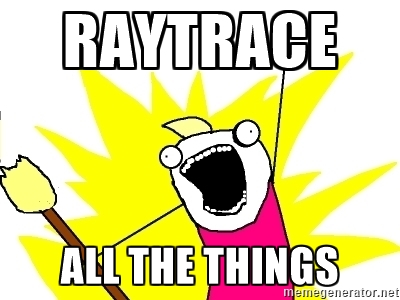
\includegraphics[width=0.5\textwidth]{raytrace_all_the_things}
	\caption*{A slide from \textit{Under the Sea: Making of "Finding Dory"}}
\end{figure}

Checking the time constantly, you reluctantly get up in time to head for your noon shift and leave as a lead character rigger begins to explain the technical difficulties involved in animating the mischievious, tentacled Hank. You think as you are leaving Hall B that not being good at drawing is an insecurity you would like to dispel over the coming year.

Worn down from a day spent putting VR headsets on people's heads, taking them off, cleaning them, and putting them on again, you grab another Starbucks Bistro box and sit dazed in the SV office with the other volunteers, watching groups head off to the RenderMan party at another hotel that you will not be venturing to this evening. In an hour, you begin to usher a couple thosuand attendees into the Computer Animation Festival's second showing from 8pm to 10pm. You figure this isn't the worst thing to happen, as you loved the first showing and your scan for recording devices during the show will let you watch most of the shorts again---some of these shorts are not even available outside this evening's showing. Realizing that the event was overstaffed, you are informed by a Team Leader part way through the show that you are free to leave or take a seat and watch the rest of the Electronic Theater.

You leave your post where you walked up and down the right side of the room scanning for recording devices in between pausing to actually watch the show. It is probably too late to head to the RenderMan party, and you would honestly like to see some of Disney and Pixar's shorts again towards the end of the show (around 10pm). You find a seat next to the video game developer you met earlier who is working on her dissertation at The University of Edinburgh. Her name is Saran. On Monday she was working at the show, so both of you are seeing most of the shorts for the second time, and it is in watching things for a second time that you can appreciate the particular elements you cherished in each short. Between shorts you take turns leaning into each other to whisper some remark about what you've seen, or to ask which ones the other liked the most and why. When the show ends, she has to leave to meet a professor of hers who is in town, so you head off on your own.

Tomorrow you plan to head to Huntington Beach after the day's shifts and programming have finished with three other friends you have joined on previous nights at receptions and local bars. You retire early to do laundry and get a good night of sleep before the next day's festivities.

\end{document}